\documentclass[12pt]{article}

\usepackage{graphicx}
\usepackage{epstopdf}


\usepackage[spanish]{babel} % silabea palabras castellanas <- Puedo poner comentarios para explicar de que va este comando en la misma línea
\selectlanguage{spanish} 

%Encoding
\usepackage[utf8]{inputenc} % Acepta caracteres en castellano
\usepackage[T1]{fontenc} % Encoding de salida al pdf

%Triunfó el mal
\usepackage[normalem]{ulem}
\useunder{\uline}{\ul}{}
\providecommand{\e}[1]{\ensuremath{\times 10^{#1}}}
\usepackage{quotmark} %Uso consistente con la RAE de comillas
\usepackage{listings} % Comandos de la terminal

\usepackage{textcomp}
\usepackage{gensymb}


%Hipertexto
\usepackage[colorlinks=true,urlcolor=blue,linkcolor=blue]{hyperref} % navega por el doc: hipertexto y links

%Aquello de las urls
\usepackage{url} 

%simbolos matemáticos
\usepackage{amsmath}
\usepackage{amsfonts}
\usepackage{amssymb}
\usepackage{physics} %Best pack

% permite insertar gráficos, imágenes y figuras, en pdf o en eps
\usepackage{graphicx}
\usepackage{epstopdf}
\usepackage{multirow}
\usepackage{float}
\usepackage[export]{adjustbox}
% geometría del documento, encabezados y pies de páginas, márgenes
\usepackage[left=2cm, right=5cm, top=2cm]{geometry}
%\geometry{letterpaper,left=1mm}
\usepackage{comment}

%\usepackage[english]{babel}
%\usepackage[latin5]{inputenc}
% \usepackage{hyperref}
%\newdate{date}{10}{05}{2013}
%\date{\displaydate{date}}
\usepackage{setspace} 
\onehalfspacing
%\setlength{\parindent}{4em}
\setlength{\parskip}{1em}
\renewcommand{\baselinestretch}{2.0}
\begin{document}
\title{Cúmulos Abiertos \\ Taller 7: Ejercicio DAOMATCH y DAOFIND}

\author{
\textbf{Javier Alejandro Acevedo Barroso\thanks{e-mail: \texttt{ja.acevedo12@uniandes.edu.co}}}\\
\textit{Universidad de los Andes, Bogotá, Colombia}\\
 }% Hasta aquí llega el bloque "author" (son dos autores por informe, orden alfabético)

\date{\today}
%\date{Versión $\alpha \beta$ fecha del documento}
\maketitle %Genera el título del documento


\normalsize
\newpage




\section{Generación del archivo \emph{.raw}}
El objetivo del ejercicio es obtener un catálogo de estrellas a partir de los archivos de fotometría del ejercicio de DAOMATCH/DAOFIND. Se parte de 99 archivos con datos de fotometría para un campo. Haciendo uso del software de Peter Stetson \tqt{DAOMATCH} y \tqt{DAOMASTER}, se puede obtener a partir de los archivos de fotometría un archivo \tqt{.raw} con las magnitudes y errores de cada estrella en cada archivo. En este informe se retratará como generar el archivo \tqt{.raw} y se propondrá un pseudo-código para obtener un catálogo a partir del archivo.

El primer paso es encontrar cuál de los cien archivos de fotometrías contiene más estrellas. Para esto se utiliza comandos de la bash para listar el número de estrellas por archivo y el nombre del archivo, una vez listados, se elije manualmente el más alto.

\begin{lstlisting}[language=bash]
  $ tail *.out -n 1
\end{lstlisting}

Se generará una lista donde la primera entrada es el nombre de un archivo de fotometría y la segunda entrada es la última línea de dicho archivo. La tercera entrada es el nombre de otro archivo de fotometría y así sucesivamente. EL primer número de la segunda línea corresponde a al número de estrellas en el archivo, de modo que solo es mirar \tqt{a ojo} cual es archivo con más estrellas. Se encontró que el archivo con más estrellas es \tqt{WFIB351\_6.OUT} con 4649 estrellas.

Usando a \tqt{WFIB351\_6.OUT} como master file, se ejecuta DAOMATCH. Agregando uno por uno cada archivo de fotometría del ejercicio (99 archivos), se obtiene al final un archivo \tqt{WFIB351\_6.mch} con las transformaciones de coordenadas para cada archivo de fotometría respecto a \tqt{WFIB351\_6.OUT}.

Ya teniendo un archivo de transformación, se procede a utilizar DAOMASTER. Este programa toma el archivo de transformación, que fue generado con solo las 30 estrellas más brillantes, y repite el análisis con la mayor cantidad de estrellas posibles. Adicionalmente, DAOMASTER permite filtrar las estrellas de interés de acuerdo al número de frames en el que aparecen (archivos de fotometría) y la fracción de frames en las que aparecen. Rememorando lo discutido en clase, se utiliza como parámetros: 30, 0.5, 98.
Tales parámetros implican que para que una estrella sea incluida en el catálogo debe estar mínimo en 30 imágenes, debe estar en mínimo la mitad de los frames,  y que si una estrella está en 98 de los frames es automáticamente incluida sin importar qué.

Tras darle los parámetros a DAOMASTER, este pregunta por el tipo de output a guardar. En esta selección siempre se procura guardar al menos el archivo \tqt{.raw} pues es el que permite hacer el catálogo.

\section{Código para la creación del catálogo}
Por último, se propone un mini codigo para obtener el catálogo a partir del \tqt{.raw} usando python.


\begin{lstlisting}[language=python]
	>>>> import numpy as np
	>>>> raw = np.loadtxt('WFIB351_6.raw')
	>>>> ids = raw[:,0]
	>>>> catalog = raw[ids == 'WFIB351_6.OUT']
	>>>> catalog.write('catalogo.txt')
\end{lstlisting}

El código toma el archivo \tqt{.raw} y retorna un catálogo con las magnitudes en el archivo de fotometría \tqt{WFIB351\_6.OUT} pues el máster y por ende el que probablemente contiene más estrellas.




%\bibliography{bibte}
\bibliographystyle{plain}


\end{document}




\begin{figure}[H]
  \centering
   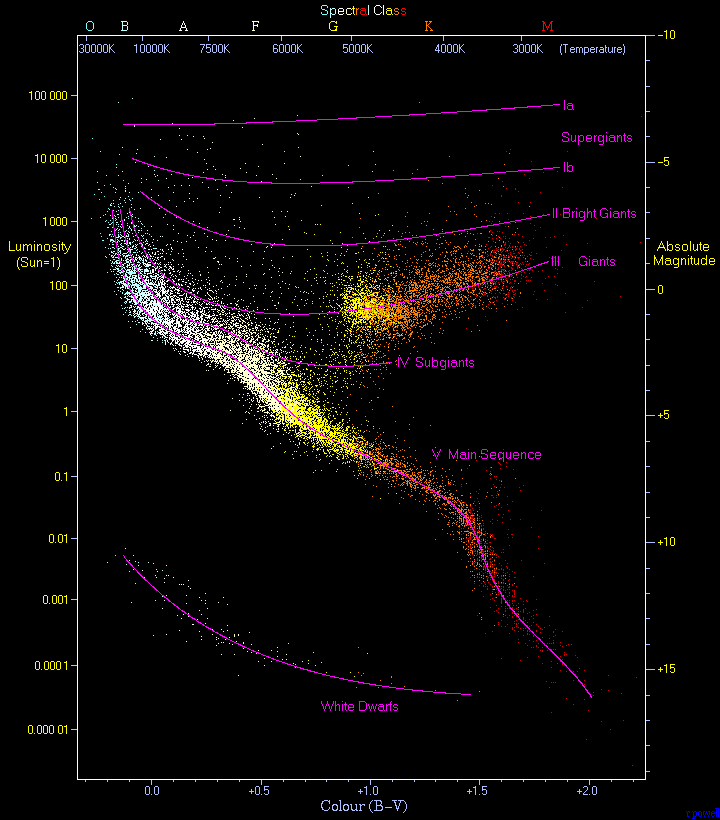
\includegraphics[width= 3.60in]{HRdiag.png}
  %\caption{Diagrama HR de 22000 estrellas del catálogo HIPPARCOS.\cite{hrdiag}  }
  \label{diag}
\end{figure}



\begin{table}[htb]
    \centering
    \label{tabla}
	\begin{tabular}{|c|c|c|c|c| }
	\hline
	Cúmulo & $E(B-V)$ & $m-M$ & Distancia [$pcs$] & Edad del cúmulo [millones de años]  \\ \hline
	NCG 752 & -0.03 & 8.02 & 401.79 & 1259  \\ \hline
	Mel 20 & +0.09 & 6.35 & 186.2 & 63  \\ \hline
	M45 & +0.04 & 5.50 & 125.89 & 126  \\ \hline
	Hyades & 0.00 & 2.84 & 36.98 & 891  \\ \hline
	M44 & +0.04 & 6.21 & 174.58 & 794  \\ \hline
	M67 & -0.03 & 9.32 & 731.14 & 5623  \\ \hline
	IC 4665 & 0.18 & 7.86 & 373.25 & 224  \\ \hline
	M39 & +0.01 & 6.87 & 238.78 & 447  \\ \hline
	\end{tabular}
\end{table}

\begin{table}[htb]
	\begin{tabular}{|c|cccccccccccccccc| }
	\hline
	Tareas $\backslash$ Semanas & 1 & 2 & 3 & 4 & 5 & 6 & 7 & 8 & 9 & 10 & 11 & 12 & 13 & 14 & 15 & 16  \\
	\hline
	1 & X & X & X  &   &   &   &   &  &  &   &   &   &   &   &   &   \\
	2 &   &  & X & X & X &  &  &   &   &  &  &  &   &  &  &   \\
	3 &   &   &   &  & X  & X  & X  & X &   &   &   &  &   &   &  &   \\
	4 &  &  &  &  &  &  &  & X & X & X & X &   &   &   &   &   \\
    5 &  &  &  &  &  &  & X & X &  &  &  &   &   &   &   &   \\
	6 &   &   &   &   &  &   &  X & X  &  &   &  X & X &  X & X  & X &   \\
	\hline
	\end{tabular}
\end{table}
\vspace{1mm}
%CCDRED se encarga de la corrección en sí, sus parámetros son: el tipo de dato de los pixeles (real, short, etc), el nombre del backup (en caso de querer un backup), el archivo de traducción del instrumento (que para una CCD estandar ya viene incluido en IRAF